\chapter{Data Management}
\Authors{Carolin Helbig et al.}

Data management includes the development and use of architectures, guidelines, practices and procedures for accurate managing of data during the entire data lifecycle of an institutional unit or a research project. Data are defined as different information units such as numbers, alphabetic characters, and symbols that are particularly formatted and can be processed by computer. The data in the project is provided by various actors which can be GeomInt partners, their legal representatives, employees, and external partners. GeomInt Data is provided at GeomInt data management portal (DMP).

In GeomInt project the partners work is very close cooperation. Project-owned and connected infrastructures are synergetic used (as illustrated in Fig. \ref{fig:geomint-dms}). In addition to the rock mechanics laboratories of the partners CAU, IfG and TUBAF with partly unique equipment data from ongoing experiments in the underground laboratories are accessed. An essential element of the GeomInt project is the simulation and software development structures illustrated in Fig. \ref{fig:geomint-dms}. With regard to the use of the simulation platform OpenGeoSys, the development of which is coordinated by the UFZ and in whose further development the GeomInt partners BGR, CAU, IfG and TUBAF are involved, the simulation and development infrastructures located at the UFZ, including version management, is available to these partners. 

%\begin{figure}{l}{\textwidth}
\begin{figure}
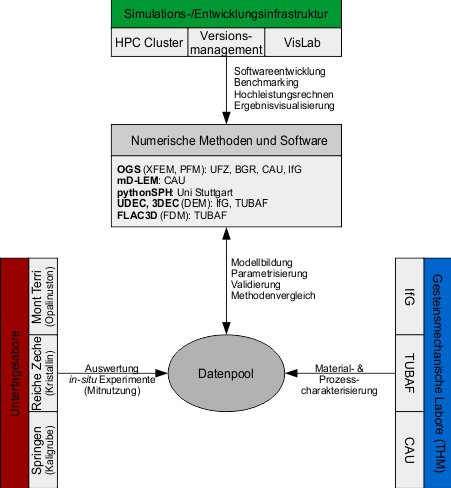
\includegraphics[width=\textwidth]{figures/geomint-dms.png}
\caption{Network diagram to illustrate synergies and dependencies in the GeomInt network in connection with the infrastructure elements and numerical methods in the project}
\label{fig:geomint-dms}
\end{figure}

The collaborative work requires data management structures and guidelines. Therefore, the first step was to set up a document that includes a user agreement and a data management plan which is the basis for data management in the project.

% The synergetic use of project-owned and connected infrastructures is illustrated in Fig. \ref{fig:geomint-dms}. In addition to the rock mechanics laboratories of the partners CAU, IfG and TUBAF with partly unique equipment (e.g. large shear apparatus of TUBAF, crack detection by means of sound waves by CAU and TUBAF, especially triax cells for percolation experiments at high temperatures at IfG), data from ongoing experiments in the above-mentioned underground laboratories are accessed. An essential element of the GeomInt project is the simulation and software development structures illustrated in Fig. \ref{fig:geomint-dms}. With regard to the use of the simulation platform OpenGeoSys, the development of which is coordinated by the UFZ and in whose further development the GeomInt partners BGR, CAU, IfG and TUBAF are involved, the simulation and development infrastructures located at the UFZ, including version management, is available to these partners.

% The immediate project results include specific data from laboratory and in-situ experiments, software components and data sets from numerical simulations (i.e. model and result files). An estimation of the extent of the data generated in GeomInt is variable; therefore, the data management concept must be flexible. This uncertainty is mainly due to the fact that the evaluation of test and calculation results may lead to a change in test and calculation planning and may even lead to additional experiments or simulation calculations. As a measure for the expected orders of magnitude, however, it is possible, for example, to estimate the size of the data set (input and output data) for the three-dimensional simulation of a transient coupled process in relation to an in-situ experiment (small field scale) with a gigabyte amount in the low two-digit range. A total data volume in the terrabyte range therefore must be manageable.

% The availability of experimental and numerical data generated in the project, including existing metadata, is realised for the project partners in an internal area of the Geomint homepage. The Helmholtz Centre for Environmental Research - UFZ is responsible for the project data. The UFZ has many years of experience in data management regarding the cooperative development of open source software (OpenGeoSys) as well as the acquisition, storage and processing of data from experiments on different scales, exploration and monitoring campaigns, numerical simulations and scientific 3D visualisations. The UFZ has sufficient capacities and modern data management systems for data storage, which are available as a central data infrastructure for the planned research network. Specifically, data sets are managed by means of an ORACLE database. Access is via a web portal, where each data record must be provided with metadata before uploading. The metadata standard used is compatible with the INSPIRE Directive 2007/2/EC and also regulates the rights for access, use and transfer of the data. A tape system is also available for the long-term storage of very large amounts of data. For the provision of exploration and monitoring data, geo-services mentioned in the GDI-DE are used as far as possible (e.g. Sensor Observation Service or Web Map Service). Since such services for complex modelling and simulation data do not exist so far, the provision is done via a data research portal, where data can be found by means of stored metadata. 

% As software components are part of non-commercial, scientific program platforms and are open source products (e.g. OpenGeoSys), they are hosted by the responsible partner via established source code hosting services (e.g. GitHub) is made publicly available. A possible public access to project data, which goes beyond the status quo as described in technical publications, as well as the handling of the data after the end of the project is regulated in the cooperation agreement or in the cooperation contract between the project partners. The handling of data obtained from the in-situ experiments in the underground laboratories through synergies with other projects is also regulated separately (access authorisation for these data, storage location, publication, handling of the data after the end of the project). Such an approach is necessary because specific parts of these data can be used for the scientific purposes of GeomInt, but they are generated in other projects with partly other partners.

\section{User agreement and data management plan}

The GeomInt project partners agreed to set up a user agreement which includes specifications for data structures including metadata, data formats, access authorization for data, the possible publication of data, as well as the handling of the data after the end of the project and outside the project. A first version of this user agreement was created six months after the start of the project. 

The user agreement includes guidelines and definitions for the following aspects 

\begin{list}{-}{\leftmargin=1em \itemindent=0em \itemsep=0.2em}
\item Which data will be generated in the project and has to be managed?
\item How will data be provided and exchanged?
\item What are the rights of use for the partners and for third parties?
\item How to cite data?
\item How to supervise the compliance of the user agreement?
\end{list}

As part of the user agreement, a data management plan, which is a formal document that describes how project data is managed during the research period and after completion of the project, was developed. The goal of a DMP plan is to consider the aspects of data management (metadata creation, data preservation and analysis) before the start of the project. Following points are discussed in the GeomInt DMP:

\begin{enumerate}{\leftmargin=1em \itemindent=0em \itemsep=0.2em}
\item Generation and management methods (data infrastructure, external data, data integration, data formats, quality control, user groups, data processing stages, versioning, documentation and meta data, geocoding)
\item Data Legal Management
\item Data exchange and provision, citation rules
\item Short-term storage and data management (storages, data transfer, backup, security)
\item Long-term storage (characteristics, metadata and documentation, responsibility)
\item Resources (organizational roles and responsibilities for data management)
\end{enumerate}

\section{GeomInt data}

The project results include specific data from laboratory and in-situ experiments, software components and data sets from numerical simulations (i.e. model and result files). An estimation of the extent of the data generated in GeomInt could not be made before the project. Therefore, the data management concept had to be flexible. This uncertainty was mainly due to the fact that the evaluation of test and calculation results may lead to a change in test and calculation planning and may even lead to additional experiments or simulation calculations. 

The availability of experimental and numerical data generated in the project, including existing metadata, is realized on an internal area of the Geomint homepage. The Helmholtz Centre for Environmental Research - UFZ is responsible for the project data. The UFZ has many years of experience in data management regarding the cooperative development of open source software (OpenGeoSys) as well as the acquisition, storage and processing of data from experiments on different scales, exploration and monitoring campaigns, numerical simulations and scientific 3D visualizations. 

The UFZ has sufficient capacities and modern data management systems for data storage, which are available as a central data infrastructure for the planned research network. Specifically, data sets are managed by means of an ORACLE database. Access is via a web portal, where each data record must be provided with metadata before uploading. The metadata standard used is compatible with the INSPIRE Directive 2007/2/EC and also regulates the rights for access, use and transfer of the data. A tape system is also available for the long-term storage of very large amounts of data. For the provision of exploration and monitoring data, geo-services mentioned in the GDI-DE are used as far as possible. Since such services for complex modelling and simulation data do not exist so far, the provision is done via a data research portal, where data can be found by means of stored metadata.

As software components are part of non-commercial, scientific program platforms and are open source products (e.g. OpenGeoSys), they are hosted by the responsible partner via established source code hosting services (e.g. GitHub) is made publicly available. A possible public access to project data, which goes beyond the status quo as described in technical publications, as well as the handling of the data after the end of the project is regulated in the cooperation agreement or in the cooperation contract between the project partners. 

The handling of data obtained from the in-situ experiments in the underground laboratories through synergies with other projects is also regulated separately (access authorisation for these data, storage location, publication, handling of the data after the end of the project). Such an approach is necessary because specific parts of these data can be used for the scientific purposes of GeomInt, but they are generated in other projects with partly other partners.

\begin{figure}

\includegraphics[width=\textwidth]{figures/geomint-web-01.png}
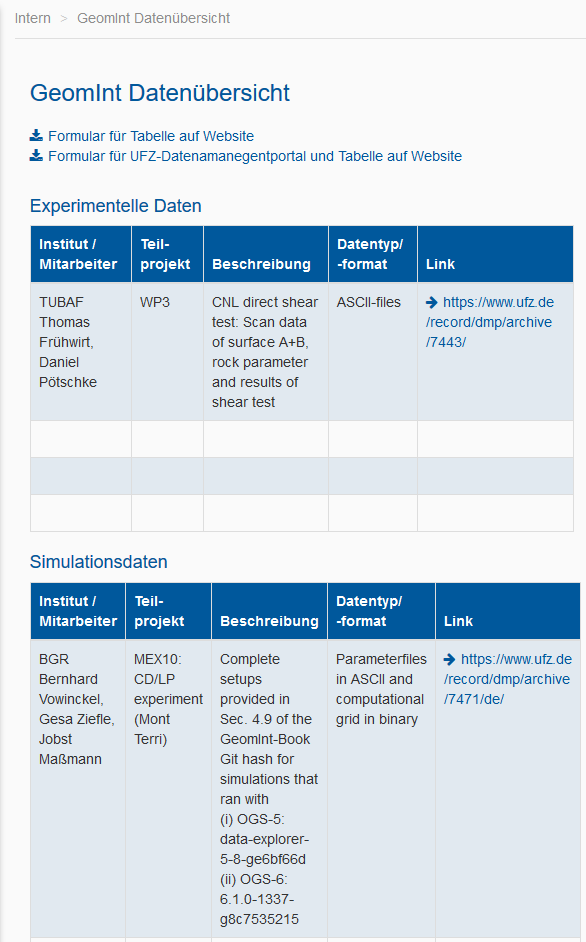
\includegraphics[width=\textwidth]{figures/geomint-web-02.png}
\caption{GeomInt DMS Portal}
\label{fig:geomint-web}
\end{figure}

\section{GeomInt DMP}

In this section, exemplary data sets of every project partner are described. A table of these data sets including description and link are available only for project partners at the website (Fig. \ref{fig:geomint-web}). Some data sets can be found on the UFZ data investigation portal \hyperlink{https://www.ufz.de/drp/}{https://www.ufz.de/drp/}. These data sets are uploaded to the data management portal at UFZ (DMP@UFZ).

\begin{table}[h!]
\footnotesize
\centering
\caption{MEX Data Management}
\label{tab:schedule}
\begin{tabular}{|C{0.6cm}|L{3.7cm}|C{0.7cm}|C{0.7cm}|C{0.7cm}|C{0.7cm}|C{0.7cm}|C{0.7cm}|} 
\hline 
\rowcolor{cyan!50}
MEX & TOP & EXP & \multicolumn{5}{c|}{MOD} \\ 
\hline
\rowcolor{cyan!50}
WP &  &  & LEM & DEM & FEM1 & FEM2 & FFS \\ 
\hline \hline
%-------------------
0-1a & Bending fracture test & REF & \cellcolor{yellow} \checkmark & \cellcolor{yellow} \checkmark & \cellcolor{yellow} \checkmark &  &  \\ 
\hline 
0-1b & Bending fracture test (aniso) & \cellcolor{yellow} & \cellcolor{yellow} & \cellcolor{yellow} & \cellcolor{yellow} &  &  \\ 
\hline 
0-2 & Humidity controlled bending & \multicolumn{6}{c|}{Concept} \\ 
\hline \hline
%-------------------
1-1a & Swelling of clay & \cellcolor{yellow} & \cellcolor{yellow} & \cellcolor{yellow} & \cellcolor{yellow} &  &  \\ 
\hline
1-1b & Swelling of clay & \cellcolor{yellow} &  & \cellcolor{yellow} &  &  &  \\ 
\hline
1-2 & Shrinkage of clay & \cellcolor{yellow} & \cellcolor{yellow} & \cellcolor{yellow} & \cellcolor{yellow} &  &  \\ 
\hline
1-3 & Desiccation of clay & \cellcolor{yellow} &  &  &  &  &  \\ 
\hline
1-4 & CD/LP experiment &  &  &  & \cellcolor{green} &  &  \\ 
\hline \hline
%-------------------
2-1a & Pressure driven percolation &  & \cellcolor{yellow} & \cellcolor{yellow} & \cellcolor{green} &  &  \\ 
\hline
2-1b & Pressure driven percolation & \cellcolor{yellow} & \cellcolor{yellow} & \cellcolor{yellow} & \cellcolor{yellow} &  &  \\ 
\hline
2-2 & Healing / closure & \cellcolor{yellow} & \cellcolor{yellow} & \cellcolor{yellow} & \cellcolor{yellow} &  &  \\ 
\hline
2-3 & Compressible fluids & \cellcolor{yellow} & \cellcolor{yellow} & \cellcolor{yellow} &  &  &  \\ 
\hline
2-4 & URL Springen & \cellcolor{yellow} &  & \cellcolor{yellow} &  &  &  \\ 
\hline \hline
%-------------------
3-1 & CNL test & \cellcolor{green} &  &  &  &  & \cellcolor{green} \\ 
\hline
3-2 & CNS test & \cellcolor{yellow} &  &  &  &  & \cellcolor{yellow} \\ 
\hline
3-3 & Cyclic loading &  &  &  &  & \cellcolor{yellow} &  \\ 
\hline \hline
%-------------------
\end{tabular}
\end{table}
\normalsize

\subsection{Software Codes}
\begin{list}{-}{\leftmargin=1em \itemindent=0em \itemsep=0.2em}
\item LEM
\item DEM: Itasca (website)
\item SPH:
\item OGS (OpenGeoSys): \url{https://www.opengeosys.org/releases/}
\item FEM@UoS: 
\end{list}
\subsection{Input files}
\begin{list}{-}{\leftmargin=1em \itemindent=0em \itemsep=0.2em}
\item LEM
\item DEM: Itasca (website)
\item SPH:
\item OGS (Benchmarks): \url{https://www.opengeosys.org/docs/benchmarks/}
\item FEM@UoS: 
\end{list}

%========================================================================
\subsection{MEX 0-1a: Bending fracture test}

Data management for MEX 0-1a (see section \ref{sec:mex01} for Model-Experiment description).

\todo[inline]{[CAU et al.]: Please add data management info for MEX 0-1a: Bending fracture test}
\todo[inline]{[UFZ](KY): Please add a template for OGS-6 (e.g. \url{https://www.opengeosys.org/docs/benchmarks/phase-field/phasefield/})}
\todo[inline]{The branch is not merged with the master yet. Files have been provided to datamanagement.}

%-------------------
\begin{table}[h!]
\footnotesize
\centering
\caption{MEX 0-1a: Data Management}
\label{tab:schedule}
\begin{tabular}{|L{0.5cm}|L{1cm}|L{2cm}|L{3cm}|L{1cm}|} 
\hline
%..................
\rowcolor{cyan!50}
 & Methods & Codes/Reference & Files & Analysis \\ \hline
 & EXP & \cite{} & Files & Analysis \\ \hline
 & LEM & Codes & Files & Analysis \\ \hline
 & DEM & UDEC & Files & Analysis \\ \hline
 & FEM & OGS-6 & Benchmark collection\footnote{\url{https://www.opengeosys.org/docs/benchmarks/phase-field/phasefield/}} & Analysis \\ \hline
%..................
\end{tabular}
\end{table}
\normalsize
%-------------------

\begin{table}[h!]
\caption{MEX 0-1a: Meta Data according to Dublin Core}
\label{tab:}
\small
\begin{tabular}{R{3cm}|L{7cm}}
\hline
%
Data label &  \\
URI &  \\
Subject  &  \\
Type of data  &  \\
Dataquality  &  \\
Status of data  &  \\
Dataformat  & \\
Creators  &  \\
Source/Origin &  \\
Publisher  &  \\
Rights holders &  \\
Contributors &  \\
Time or Period of creation &  \\
Language of the content &  \\
Update policy &  \\
Access permissions &  \\
%
\hline
\end{tabular}
\end{table}

\subsection{MEX 0-1b: Three-Point fracture toughness test on the Opalinus Claystone (CAU Kiel)}

The experimental results of the three-Point fracture toughness test on the Opalinus Claystone samples are uploaded to the IfG (Kiel) NextCloud server. The data is accessible through the following link:\\
\hyperlink{https://nextcloud.ifg.uni-kiel.de/index.php/s/pJxp2eNEJb6PfiS}{https://nextcloud.ifg.uni-kiel.de/index.php/s/pJxp2eNEJb6PfiS}\\

The data set, which includes the time, applied force($N$) and the displacement of the sample at the loading point ($mm$), is provided in a *.txt file. The crack mouth opening displacement (CMOD), which is determined from the image processing technique (section \ref {sec:Fracture_Toughness_Exp}), is given in a *.xlsx file. The data includes the time and the calculated CMOD (mm). Figure \ref{fig:Amir_Fracture_Toughness_Result_20_Data} shows the relation between the applied loading force and CMOD as described in section \ref {sec:Fracture_Toughness_Exp}.

\begin{figure}[!ht]
\centering
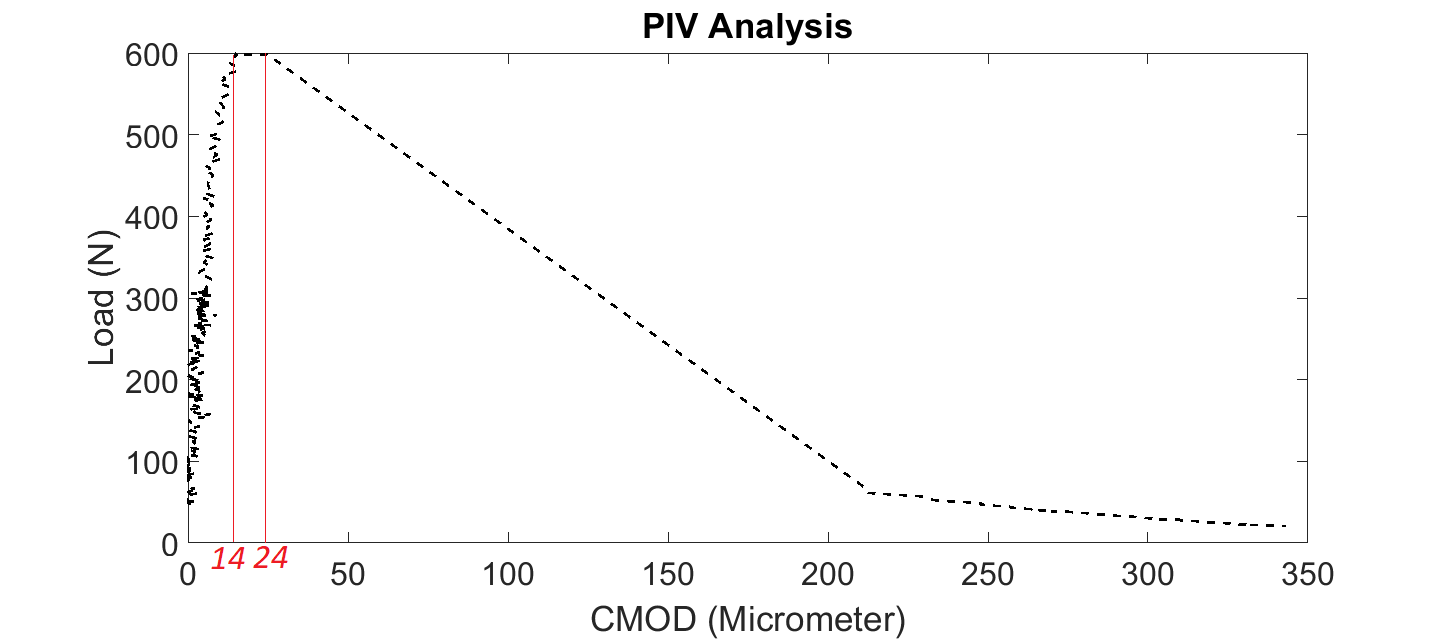
\includegraphics[width=0.75\textwidth]{figures/Amir_Fracture_Toughness_Result_20_Data.png}
\caption{The load vs. crack mouth opening displacement (CMOD) response of the Opalinus claystone}
\label{fig:Amir_Fracture_Toughness_Result_20_Data}
\end{figure}

\begin{table}[h!]
\caption{MEX 0-1b: Meta Data according to Dublin Core}
\label{tab:}
\small
\begin{tabular}{R{3cm}|L{7cm}}
\hline
%
Data label &  \\
URI &  \\
Subject  &  \\
Type of data  &  \\
Dataquality  &  \\
Status of data  &  \\
Dataformat  & \\
Creators  &  \\
Source/Origin &  \\
Publisher  &  \\
Rights holders &  \\
Contributors &  \\
Time or Period of creation &  \\
Language of the content &  \\
Update policy &  \\
Access permissions &  \\
%
\hline
\end{tabular}
\end{table}

\subsection{MEX 1-1a:}

Data management for MEX 1-1a (see \ref{sec:mex05}).
\todo[inline]{[CAU et al.]: Please add data management info for MEX 1-1a}

\begin{table}[h!]
\caption{MEX 1-1a: Meta Data according to Dublin Core}
\label{tab:}
\small
\begin{tabular}{R{3cm}|L{7cm}}
\hline
%
Data label &  \\
URI &  \\
Subject  &  \\
Type of data  &  \\
Dataquality  &  \\
Status of data  &  \\
Dataformat  & \\
Creators  &  \\
Source/Origin &  \\
Publisher  &  \\
Rights holders &  \\
Contributors &  \\
Time or Period of creation &  \\
Language of the content &  \\
Update policy &  \\
Access permissions &  \\
%
\hline
\end{tabular}
\end{table}

\subsection{MEX 1-1b:}

Data management for MEX 1-1b (see \ref{sec:mex05}).
\todo[inline]{[CAU et al.]: Please add data management info for MEX 1-1b}

\begin{table}[h!]
\caption{MEX 1-1b: Meta Data according to Dublin Core}
\label{tab:}
\small
\begin{tabular}{R{3cm}|L{7cm}}
\hline
%
Data label &  \\
URI &  \\
Subject  &  \\
Type of data  &  \\
Dataquality  &  \\
Status of data  &  \\
Dataformat  & \\
Creators  &  \\
Source/Origin &  \\
Publisher  &  \\
Rights holders &  \\
Contributors &  \\
Time or Period of creation &  \\
Language of the content &  \\
Update policy &  \\
Access permissions &  \\
%
\hline
\end{tabular}
\end{table}

\subsection{MEX 1-2: Swelling and Shrinkage of the Opalinus Claystone (CAU Kiel)}

Data management for MEX 1-2 (see \ref{sec:mex06}).

The experimental results of the shrinkage and swelling of the Opalinus Claystone are uploaded to the IfG (Kiel) NextCloud server. The data is accessible through the following link:\\
\hyperlink{https://nextcloud.ifg.uni-kiel.de/index.php/s/q6g25nWyWJKqzNB}{https://nextcloud.ifg.uni-kiel.de/index.php/s/q6g25nWyWJKqzNB}\\

The results obtained from the manual reading of the data are prepared in the *.xlsx Format. The data set includes the reading time, the axial strain of the parallel strain gauge, the axial strain of the perpendicular strain gauge, considered salt solution, corresponding suction value and the water content of the sample during the drying and wetting paths. Figure \ref{fig:Amir_Shrinkage_Strain_Data} depicts the plotted suction vs. axial strains of the claystone sample during the wetting and drying paths (section \ref{sec:Shrinkage_Swelling_Exp} and \ref{sec:mex06}).

\begin{figure}[!ht]
\centering
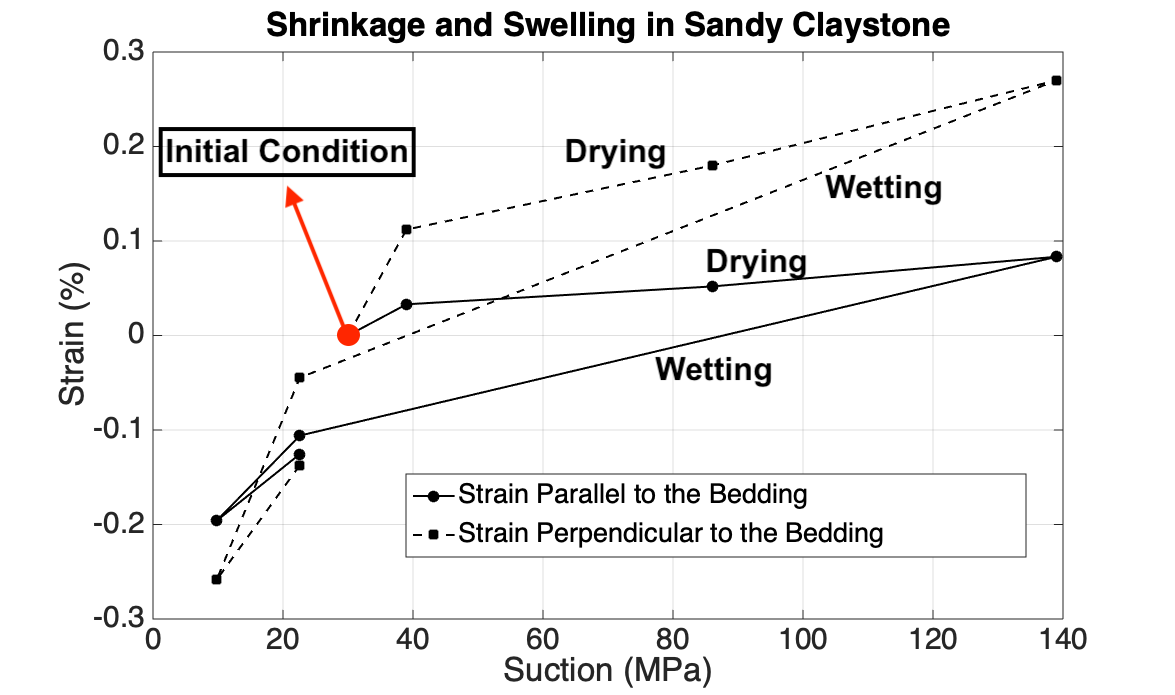
\includegraphics[width=0.5\textwidth]{figures/Amir_Shrinkage_Strain_Data.png}
\caption{The relation between the applied suction and the resultant axial strains}
\label{fig:Amir_Shrinkage_Strain_Data}
\end{figure}

\begin{table}[h!]
\caption{MEX 1-2: Meta Data according to Dublin Core}
\label{tab:}
\small
\begin{tabular}{R{3cm}|L{7cm}}
\hline
%
Data label &  \\
URI &  \\
Subject  &  \\
Type of data  &  \\
Dataquality  &  \\
Status of data  &  \\
Dataformat  & \\
Creators  &  \\
Source/Origin &  \\
Publisher  &  \\
Rights holders &  \\
Contributors &  \\
Time or Period of creation &  \\
Language of the content &  \\
Update policy &  \\
Access permissions &  \\
%
\hline
\end{tabular}
\end{table}

\subsection{MEX 1-4: CD/LP experiment (BGR)}

Data management for MEX 1-4 (see \ref{sec:mex10}).

Link to the data set at UFZ data investigation portal (Download only for project members):
\hyperlink{https://www.ufz.de/record/dmp/archive/7471/}{https://www.ufz.de/record/dmp/archive/7471/}

The data set contains all project files that are relevant to reproduce the simulation results described in Section \ref{sec:mex10} and its corresponding subsections. For every simulation run with OGS-6, the data set comprises a project file (\texttt{*.prj}), a geometry file (\texttt{*.gml}) and the computational mesh (\texttt{*.vtu}). For simulations run with OGS-5, the project is split into files for boundary conditions (\texttt{*.bc}), initial conditions (\texttt{*.ic}), fluid properties (\texttt{*.mfp}), material properties (\texttt{*.mmp}), solid properties (\texttt{*.msp}), numerical parameters (\texttt{*.num}), output parameters (\texttt{*.out}), process definitions (\texttt{*.pcs}), tabulated functional dependencies (\texttt{*.rfd}), source terms (\texttt{*.sc}), and output parameters (\texttt{*.out}). In addition, seperate files are provided for the geometry (\texttt{*.gli}) and the computational mesh (\texttt{*.msh}).

\begin{table}[h!]
\caption{MEX 1-4: Meta Data according to Dublin Core}
\label{tab:}
\small
\begin{tabular}{R{3cm}|L{7cm}}
\hline
%
Data label &  \\
URI &  \\
Subject  &  \\
Type of data  &  \\
Dataquality  &  \\
Status of data  &  \\
Dataformat  & \\
Creators  &  \\
Source/Origin &  \\
Publisher  &  \\
Rights holders &  \\
Contributors &  \\
Time or Period of creation &  \\
Language of the content &  \\
Update policy &  \\
Access permissions &  \\
%
\hline
\end{tabular}
\end{table}

\subsection{MEX 2-1a: Pressure driven percolation (salt)}

Data management for MEX 2-1a (see \ref{sec:mex02}).

Link to the data set at UFZ data investigation portal (Download only for project members):
\hyperlink{https://www.ufz.de/record/dmp/archive/7706/}{https://www.ufz.de/record/dmp/archive/7706/}.

The link contains two input decks for OGS-6 in which pressure driven percolation as described in MEX2 is simulated under different configurations of boundary loading.
The first case applies the boundary loading of 12 MPa, 21 MPa, and 8 MPa in x-, y-, and z-direction respectively. It is called ''case 1" and the corresponding OGS-6 input file is ''me2\_insitu\_case1.prj".
The second case is loaded with 4 MPa, 15 MPa, and 19 MPa in x-, y-, and z-direction respectively and the input file is named ''me2\_insitu\_case2.prj".
The remaining files are vtu files that describe the computing domain and the boundaries as shown in~\ref{fig:VPF_init}.

\begin{table}[h!]
\caption{MEX 2-1a: Meta Data according to Dublin Core}
\label{tab:}
\small
\begin{tabular}{R{3cm}|L{7cm}}
\hline
%
Data label &  \\
URI &  \\
Subject  &  \\
Type of data  &  \\
Dataquality  &  \\
Status of data  &  \\
Dataformat  & \\
Creators  &  \\
Source/Origin &  \\
Publisher  &  \\
Rights holders &  \\
Contributors &  \\
Time or Period of creation &  \\
Language of the content &  \\
Update policy &  \\
Access permissions &  \\
%
\hline
\end{tabular}
\end{table}

\subsection{MEX 2-1b: Pressure driven percolation on the Opalinus claystone (CAU Kiel)}

Data management for MEX 2-1b (see \ref{sec:mex2-1b}).

The experimental results of the pressure driven percolation test on the cubic claystone samples are uploaded to the IfG (Kiel) NextCloud server. The data is accessible through the following link:\\
\hyperlink{https://nextcloud.ifg.uni-kiel.de/index.php/s/EMdNkdF4PRKWCqa}{https://nextcloud.ifg.uni-kiel.de/index.php/s/EMdNkdF4PRKWCqa}\\

The experimental data (*.ASCII) of the three different stress configurations (section \ref{sec:Percolation_Claystone_Exp}) are uploaded to the server. The data includes the time ($\Delta T=1s$), pump volume ($mL$), given oil pressure ($Bar$) and actual oil pressure in the system ($Bar$). Figure \ref{fig:Amir_Percolation_Time_Pressure1_Data}
illustrates an example of the plotted borehole pressure vs. time data for the 1st stress configuration discussed in the (section \ref{sec:Percolation_Claystone_Exp} and \ref{sec:mex02}).

\begin{figure}[!ht]
\centering
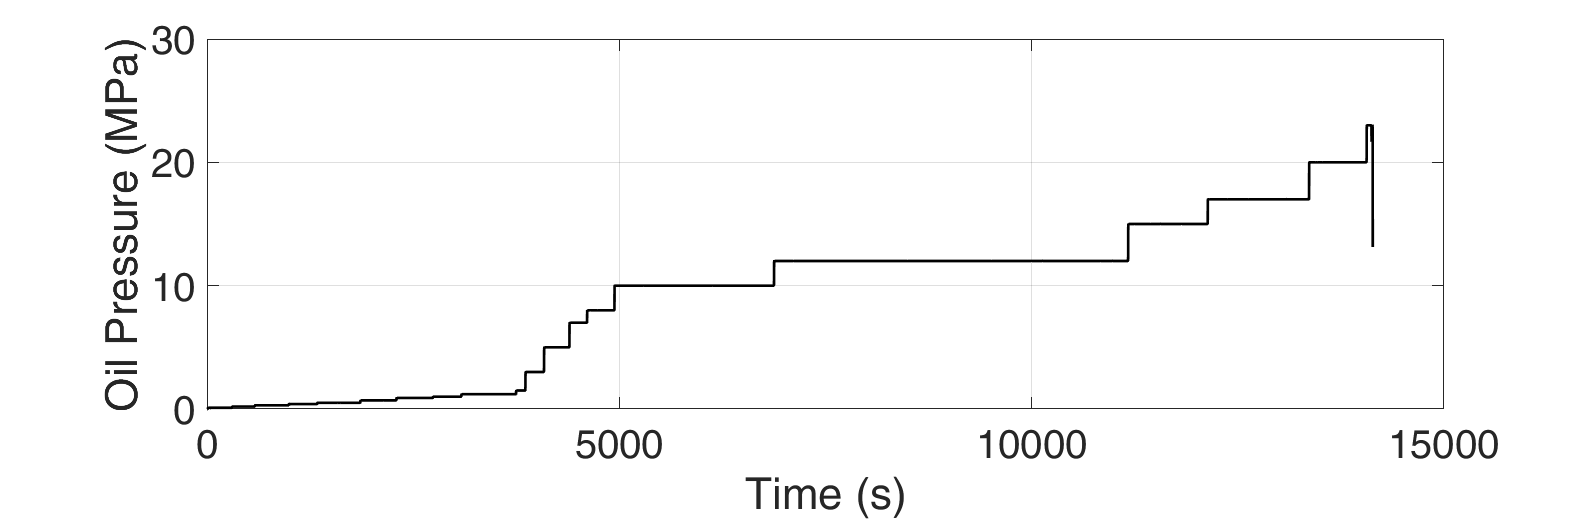
\includegraphics[width=0.75\textwidth]{figures/Amir_Percolation_Time_Pressure1_Data.png}
\caption{The recorded results depicting the evolution of the borehole pressure vs. time for the stress configuration given as \ref{fig:Amir_Percolation_Stress_1}}
\label{fig:Amir_Percolation_Time_Pressure1_Data}
\end{figure}

\begin{table}[h!]
\caption{MEX 2-1b: Meta Data according to Dublin Core}
\label{tab:}
\small
\begin{tabular}{R{3cm}|L{7cm}}
\hline
%
Data label &  \\
URI &  \\
Subject  &  \\
Type of data  &  \\
Dataquality  &  \\
Status of data  &  \\
Dataformat  & \\
Creators  &  \\
Source/Origin &  \\
Publisher  &  \\
Rights holders &  \\
Contributors &  \\
Time or Period of creation &  \\
Language of the content &  \\
Update policy &  \\
Access permissions &  \\
%
\hline
\end{tabular}
\end{table}

\subsection{MEX 2-2: Closure and healing of cracks}

Data management for MEX 2-2 (see \ref{sec:mex03}).
\todo[inline]{[IfG et al.]: Please add data management info for MEX 2-2}

The measured gas flow is converted into permeabilities, which are stored as time series in an Excel file. For each of the three experiment there are two columns. The first contains the time in hours since the start of the experiment, the second contains the permeability. 

\begin{figure}[!ht]
\centering
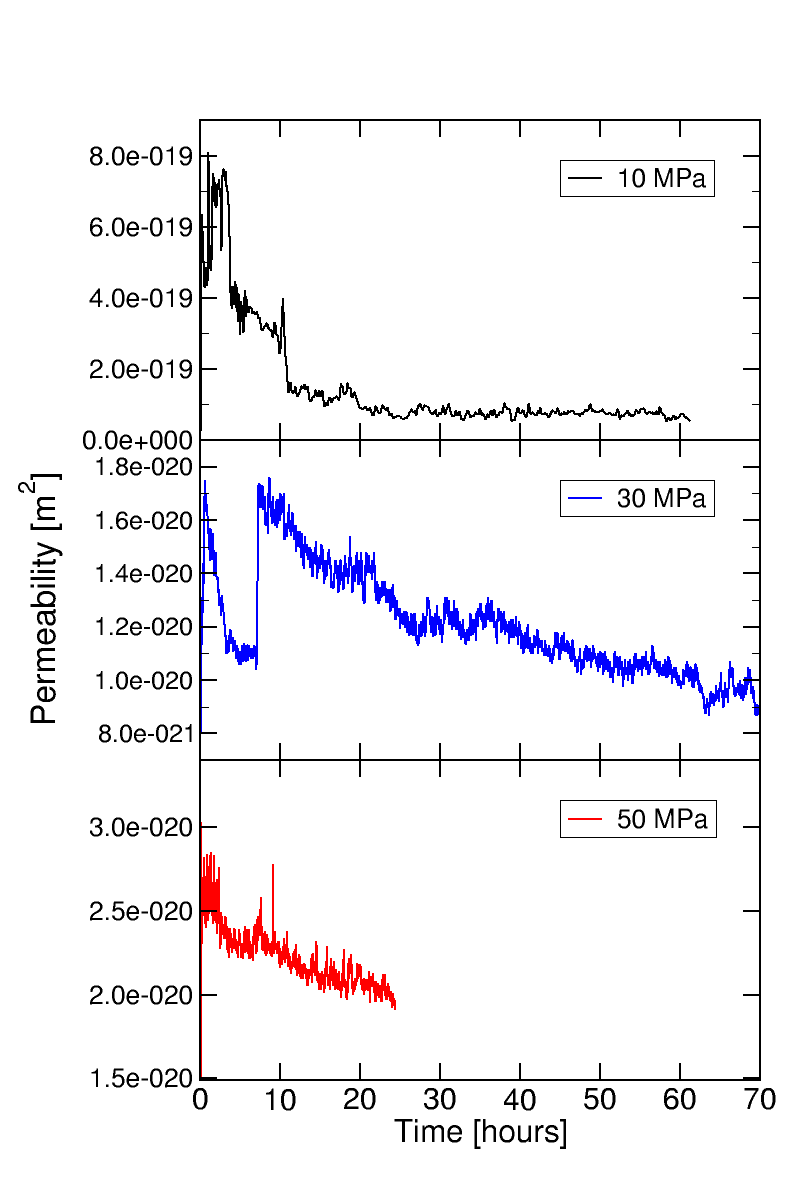
\includegraphics[width=0.5\textwidth]{figures/mex3-perme-time-comparison.png}
\caption{Graphical Representation of data.}
\label{fig:ME3-perme-exp-dmp}
\end{figure}

\begin{table}[h!]
\caption{MEX 2-2: Meta Data according to Dublin Core}
\label{tab:}
\small
\begin{tabular}{R{3cm}|L{7cm}}
\hline
%
Data label &  \\
URI &  \\
Subject  &  \\
Type of data  &  \\
Dataquality  &  \\
Status of data  &  \\
Dataformat  & \\
Creators  &  \\
Source/Origin &  \\
Publisher  &  \\
Rights holders &  \\
Contributors &  \\
Time or Period of creation &  \\
Language of the content &  \\
Update policy &  \\
Access permissions &  \\
%
\hline
\end{tabular}
\end{table}

\subsection{MEX 2-3: Effect of compressibility on pressure driven percolation}

Data management for MEX 2-3 (see \ref{sec:mex04}).
\todo[inline]{[IfG et al.]: Please add data management info for MEX 2-3}

\begin{table}[h!]
\caption{MEX 2-3: Meta Data according to Dublin Core}
\label{tab:}
\small
\begin{tabular}{R{3cm}|L{7cm}}
\hline
%
Data label &  \\
URI &  \\
Subject  &  \\
Type of data  &  \\
Dataquality  &  \\
Status of data  &  \\
Dataformat  & \\
Creators  &  \\
Source/Origin &  \\
Publisher  &  \\
Rights holders &  \\
Contributors &  \\
Time or Period of creation &  \\
Language of the content &  \\
Update policy &  \\
Access permissions &  \\
%
\hline
\end{tabular}
\end{table}

\subsection{MEX 2-4: Large wellbore test (Springen)}

Data management for MEX 2-4 (see \ref{sec:mex11}).
\todo[inline]{[IfG]: Please add data management info for MEX 2-4}

\begin{table}[h!]
\caption{MEX 2-4: Meta Data according to Dublin Core}
\label{tab:}
\small
\begin{tabular}{R{3cm}|L{7cm}}
\hline
%
Data label &  \\
URI &  \\
Subject  &  \\
Type of data  &  \\
Dataquality  &  \\
Status of data  &  \\
Dataformat  & \\
Creators  &  \\
Source/Origin &  \\
Publisher  &  \\
Rights holders &  \\
Contributors &  \\
Time or Period of creation &  \\
Language of the content &  \\
Update policy &  \\
Access permissions &  \\
%
\hline
\end{tabular}
\end{table}

\subsection{MEX 3-1: CNL direct shear test data (TUBAF)}\label{DataManMex3-1CNL}\index{Constant Normal Load (CNL) experiment}

Data management for MEX 3-1 (see \ref{sec:mex07}).

Link to the data set at UFZ data investigation portal (Download only for project members):
\url{https://www.ufz.de/record/dmp/archive/7443/}

The CNL data set contains four text files. One text file with the rock properties of the used granite (see Tab. \ref{table:MEX7_rockParam}). Two files with the scan data of the two surfaces. One point cloud can be seen in Fig. \ref{fig:DataCNLGranitePointCloud}. The last file contains the laboratory data. In Fig. \ref{fig:DataCNLGraniteLab} the results for the four shear stress levels can be seen.

\begin{figure}[!ht]
\begin{center}
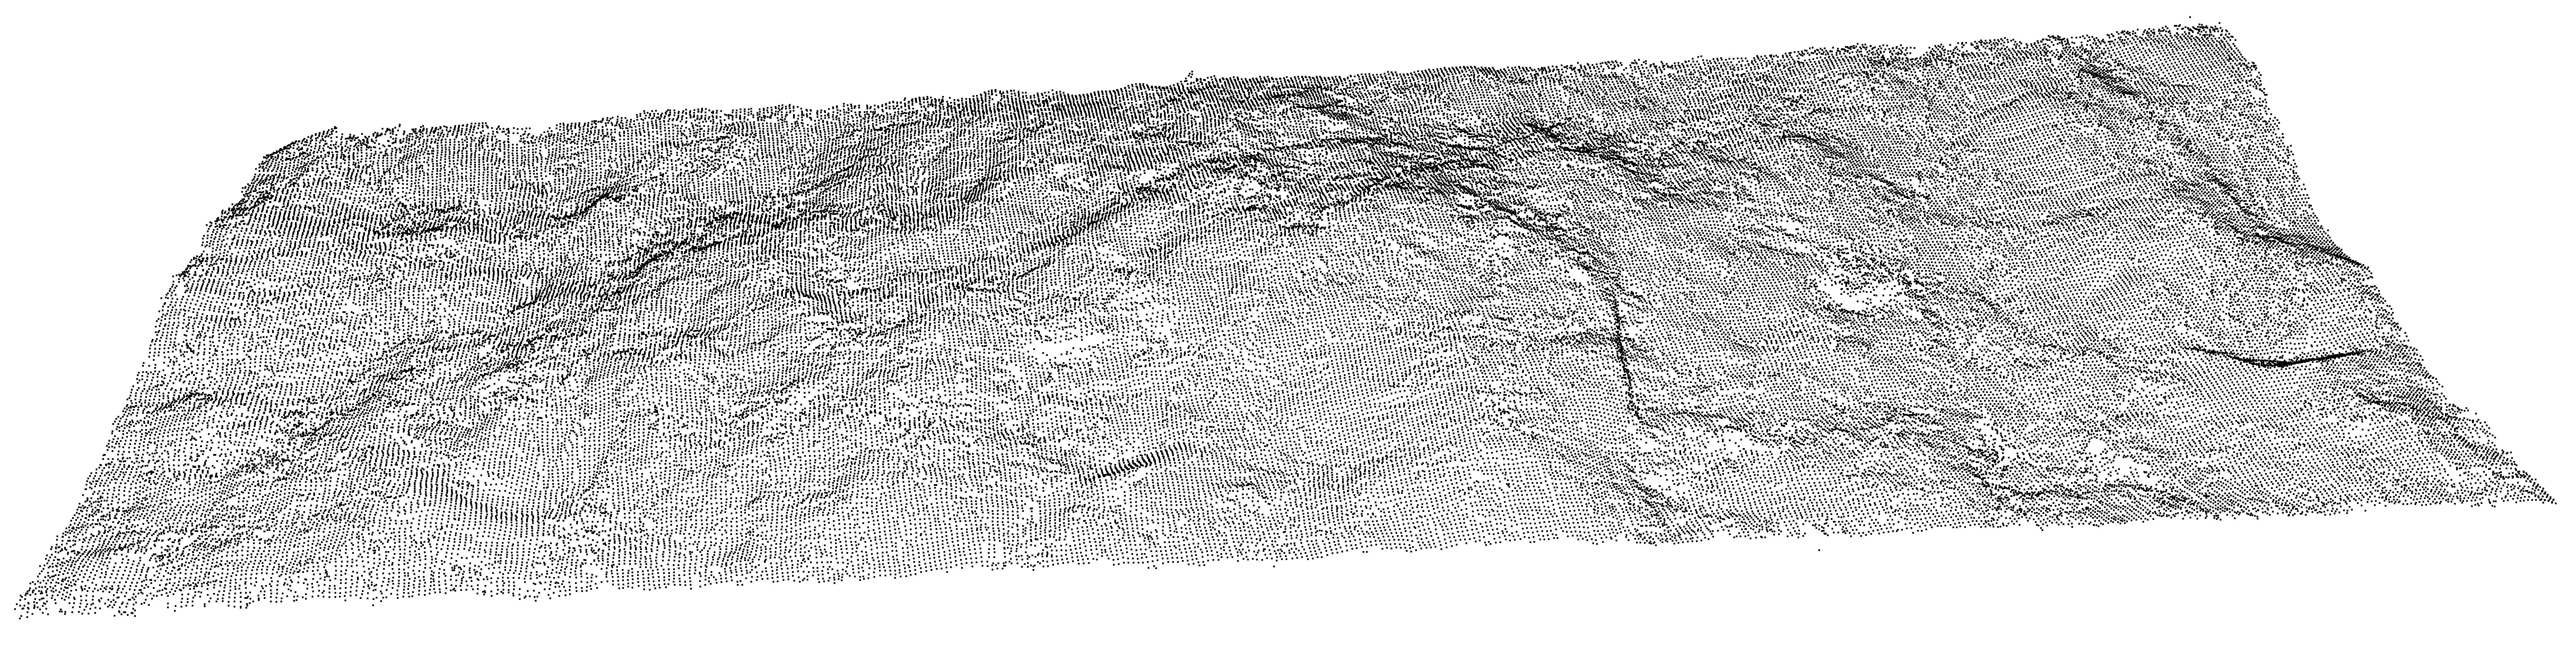
\includegraphics[width=0.5\textwidth]{./figures/MEX7_Point_cloud.png}
\end{center}
\caption{Point cloud representing the surface of a granite sample from Saxony. The size is 65 mm by 170 mm and the cloud contains approx. 98000 points.}
\label{fig:DataCNLGranitePointCloud}
\end{figure}

\begin{figure}[!ht]
\begin{tabular}{cc}
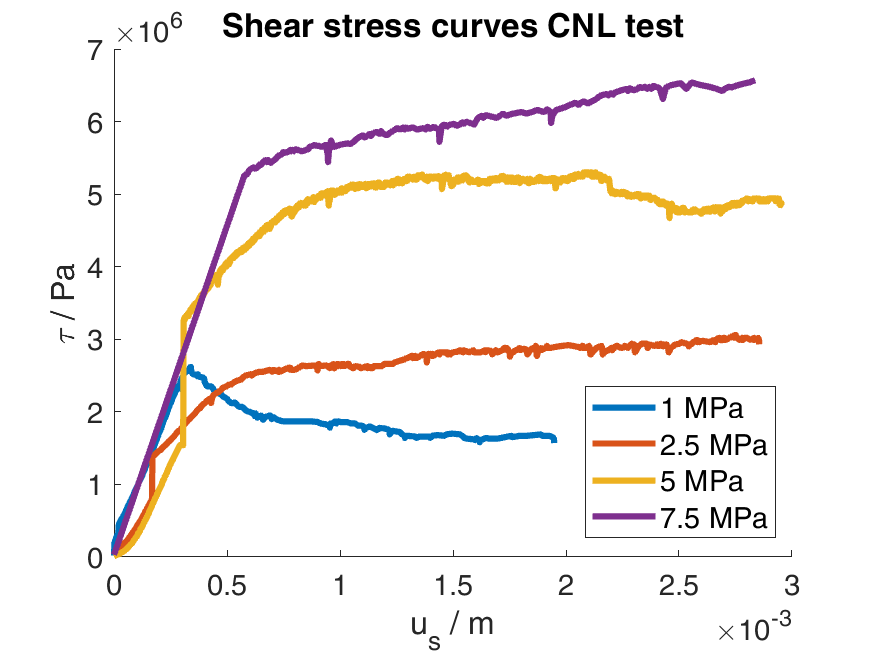
\includegraphics[width=0.45\textwidth]{./figures/CNLShearCurvesAll.png}     
& 
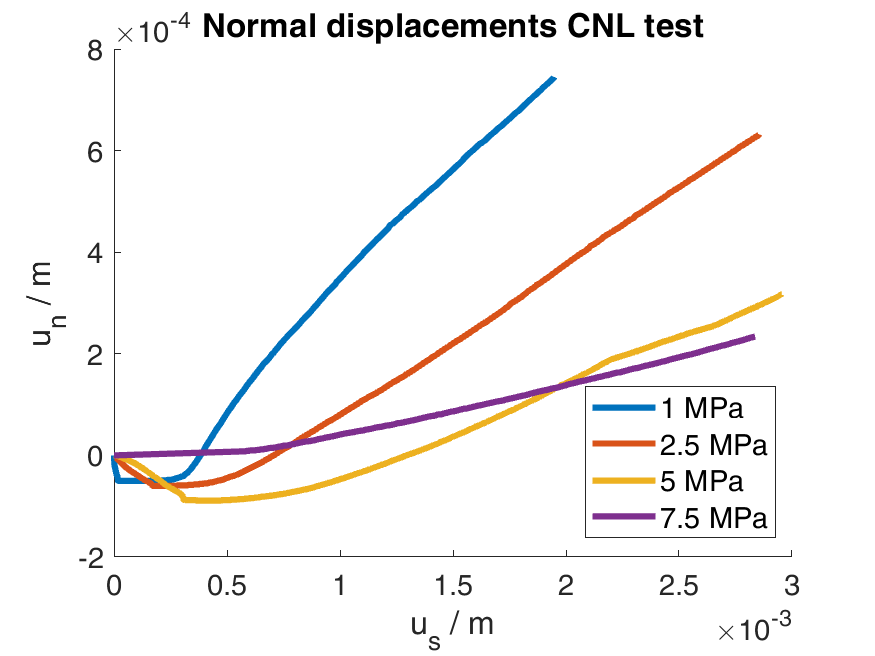
\includegraphics[width=0.45\textwidth]{./figures/CNLDilatationAll.png} 
\end{tabular}
\caption{CNL test results}
\label{fig:DataCNLGraniteLab}
\end{figure}

\begin{table}[h!]
\caption{MEX 3-1: Meta Data according to Dublin Core}
\label{tab:}
\small
\begin{tabular}{R{3cm}|L{7cm}}
\hline
%\rowcolor{Cyan}
%
Data label & GeomInt | TUBAF | Data Set CNL \\
URI & http://www.ufz.de/record/dmp/archive/7443 \\
Subject  & Crystalline rock, direct shear test \\
Type of data  & Sammlung verschiedener Daten \\
Dataquality  & qualitätsgesicherte Daten \\
Status of data  & bearbeitete Daten \\
Dataformat  & txt \\
Creators  & TU Freiberg, Institut für Geotechnik, Gustav-Zeuner-Str. 1, 09599 Freiberg \\
Source/Origin  & Rock mechanical laboratory \\
Publisher  & TU Freiberg, Institut für Geotechnik, Gustav-Zeuner-Str. 1, 09599 Freiberg \\
Rights holders  & TU Freiberg, Institut für Geotechnik, Gustav-Zeuner-Str. 1, 09599 Freiberg \\
Contributors  & TU Freiberg, Institut für Geotechnik, Thomas Frühwirt und Daniel Pötschke \\
Time or Period of creation  & 2018 - 2019 \\
Language of the content & Englisch \\
Update policy  & Der Datenbestand wird nicht erweitert \\
Access permissions  & beschränkter Zugriff \\
%
\hline
\end{tabular}
\end{table}

\subsection{MEX 3-2: CNS test}\label{DataManMex3-2CNS}\index{Constant Normal Stiffness (CNS) experiment}

Data management for MEX 3-2 (see \ref{sec:mex08}).
\todo[inline]{[TUBAF]: Please add data management info for MEX 3-2: CNS test}
The data set of the CNS test contains a file with the rock properties of the used basalt (see Tab. \ref{table:MEX7_rockParam}), two files with the scan data of the two surfaces. One point cloud can be seen in Fig. \ref{fig:DataCNSBasaltPointCloud}. The results of the laboratory tests are available as ASCII files and the shear curves and the dilatation are visualized in Fig. \ref{fig:DataCNSBasaltLab}. Additionally three photos of the basalt surface before, after the first and after the fourth shear test are included. 

\begin{figure}[!ht]
\begin{center}
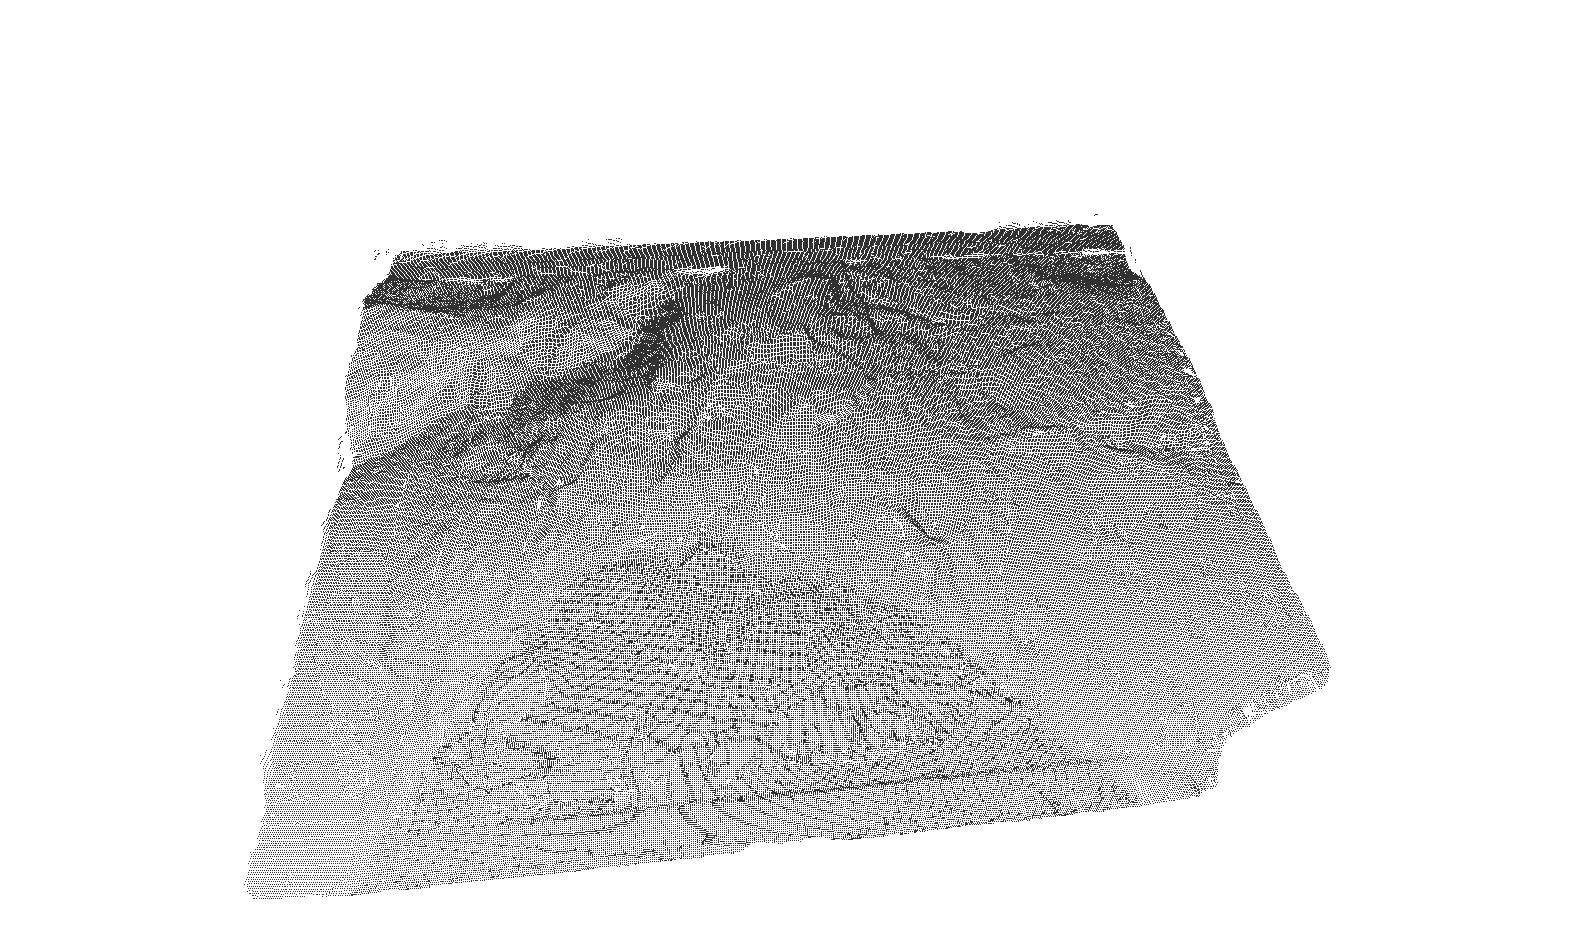
\includegraphics[width=0.5\textwidth]{./figures/MEX3-2PointCloud.png}
\end{center}
\caption{Point cloud representing the surface of a basalt sample from Thuringia. The size is 196 mm by 149 mm and the cloud contains approx. 252000 points.}
\label{fig:DataCNSBasaltPointCloud}
\end{figure}

\begin{figure}[!ht]
\begin{tabular}{cc}
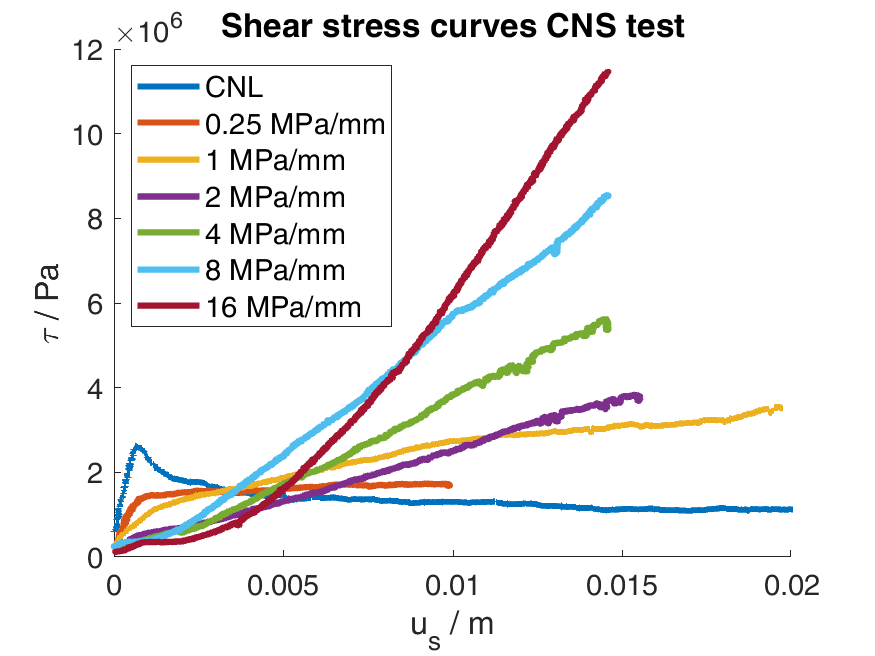
\includegraphics[width=0.45\textwidth]{./figures/CNSShearCurvesAll.png}     
& 
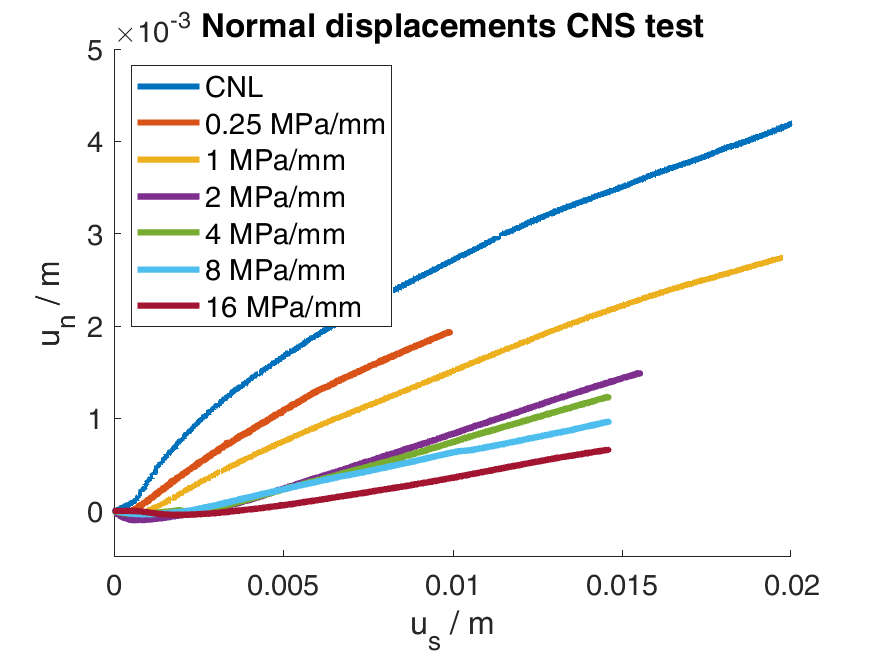
\includegraphics[width=0.45\textwidth]{./figures/CNSDilatationAll.png} 
\end{tabular}
\caption{CNL test results}
\label{fig:DataCNSBasaltLab}
\end{figure}

\begin{table}[h!]
\caption{MEX 3-2: Meta Data according to Dublin Core}
\label{tab:}
\small
\begin{tabular}{R{3cm}|L{7cm}}
\hline
%
Data label &  \\
URI &  \\
Subject  &  \\
Type of data  &  \\
Dataquality  &  \\
Status of data  &  \\
Dataformat  & \\
Creators  &  \\
Source/Origin &  \\
Publisher  &  \\
Rights holders &  \\
Contributors &  \\
Time or Period of creation &  \\
Language of the content &  \\
Update policy &  \\
Access permissions &  \\
%
\hline
\end{tabular}
\end{table}


\subsection{MEX 3-3: Cyclic loading}

Data management for MEX 3-3 (see \ref{sec:mex09}).

Link to the data set stored at the Gitlab server located at the Institute of Applied Mechanics, University of Stuttgart:\\
\hyperlink{https://galilei.isr.uni-stuttgart.de/gitlab/schmidt/geomint}{https://galilei.isr.uni-stuttgart.de/gitlab/schmidt/geomint}\\

The uploaded data set contains two compiled executables for simulations to fit experimental data for the Reichen Zeche fracture characterization tests and to reproduce the non-linear response throughout harmonic testing of a single fracture on the laboratory scale like described in section \ref{sec:mex09}. The folder includes executables, input files and the used discretization in terms of meshing files, required to perform the simulations. README.txt files provide further informations how to start the simulations.

\begin{table}[h!]
\caption{MEX 3-3: Meta Data according to Dublin Core}
\label{tab:}
\small
\begin{tabular}{R{3cm}|L{7cm}}
\hline
%
Data label &  \\
URI &  \\
Subject  &  \\
Type of data  &  \\
Dataquality  &  \\
Status of data  &  \\
Dataformat  & \\
Creators  &  \\
Source/Origin &  \\
Publisher  &  \\
Rights holders &  \\
Contributors &  \\
Time or Period of creation &  \\
Language of the content &  \\
Update policy &  \\
Access permissions &  \\
%
\hline
\end{tabular}
\end{table}